
\cvsid{$Id$}

\chapter{Grafika, tablice i bibliografia}
% \chaptermark{Tytuł skrócony można pominąć\ldots{}}{}

\section{Wstawianie rysunków}

Program \texttt{latex} używa rysunków w postaci plików EPS. Program \texttt{pdflatex}
potrafi włączać do dokumentu rysunki zarówno pliki bitmapowe (PNG, JPG),
jak i inne pliki PDF. Polecam ten drugi.

Rysunki umieszcza się u góry strony (\LaTeX{} sam zwykle o to zadba). Nie należy przejmować
się jeśli rysunek przeniesie się na następną stronę. Odwołania do rysunków
tworzy się przy pomocy poleceń \texttt{ref}, \texttt{pageref} i \texttt{label}.
Przykładowo, rysunek~\ref{rys:cwpp} na stronie~\pageref{rys:cwpp} przedstawia
reaktor.

\begin{figure}[t]
\begin{center}
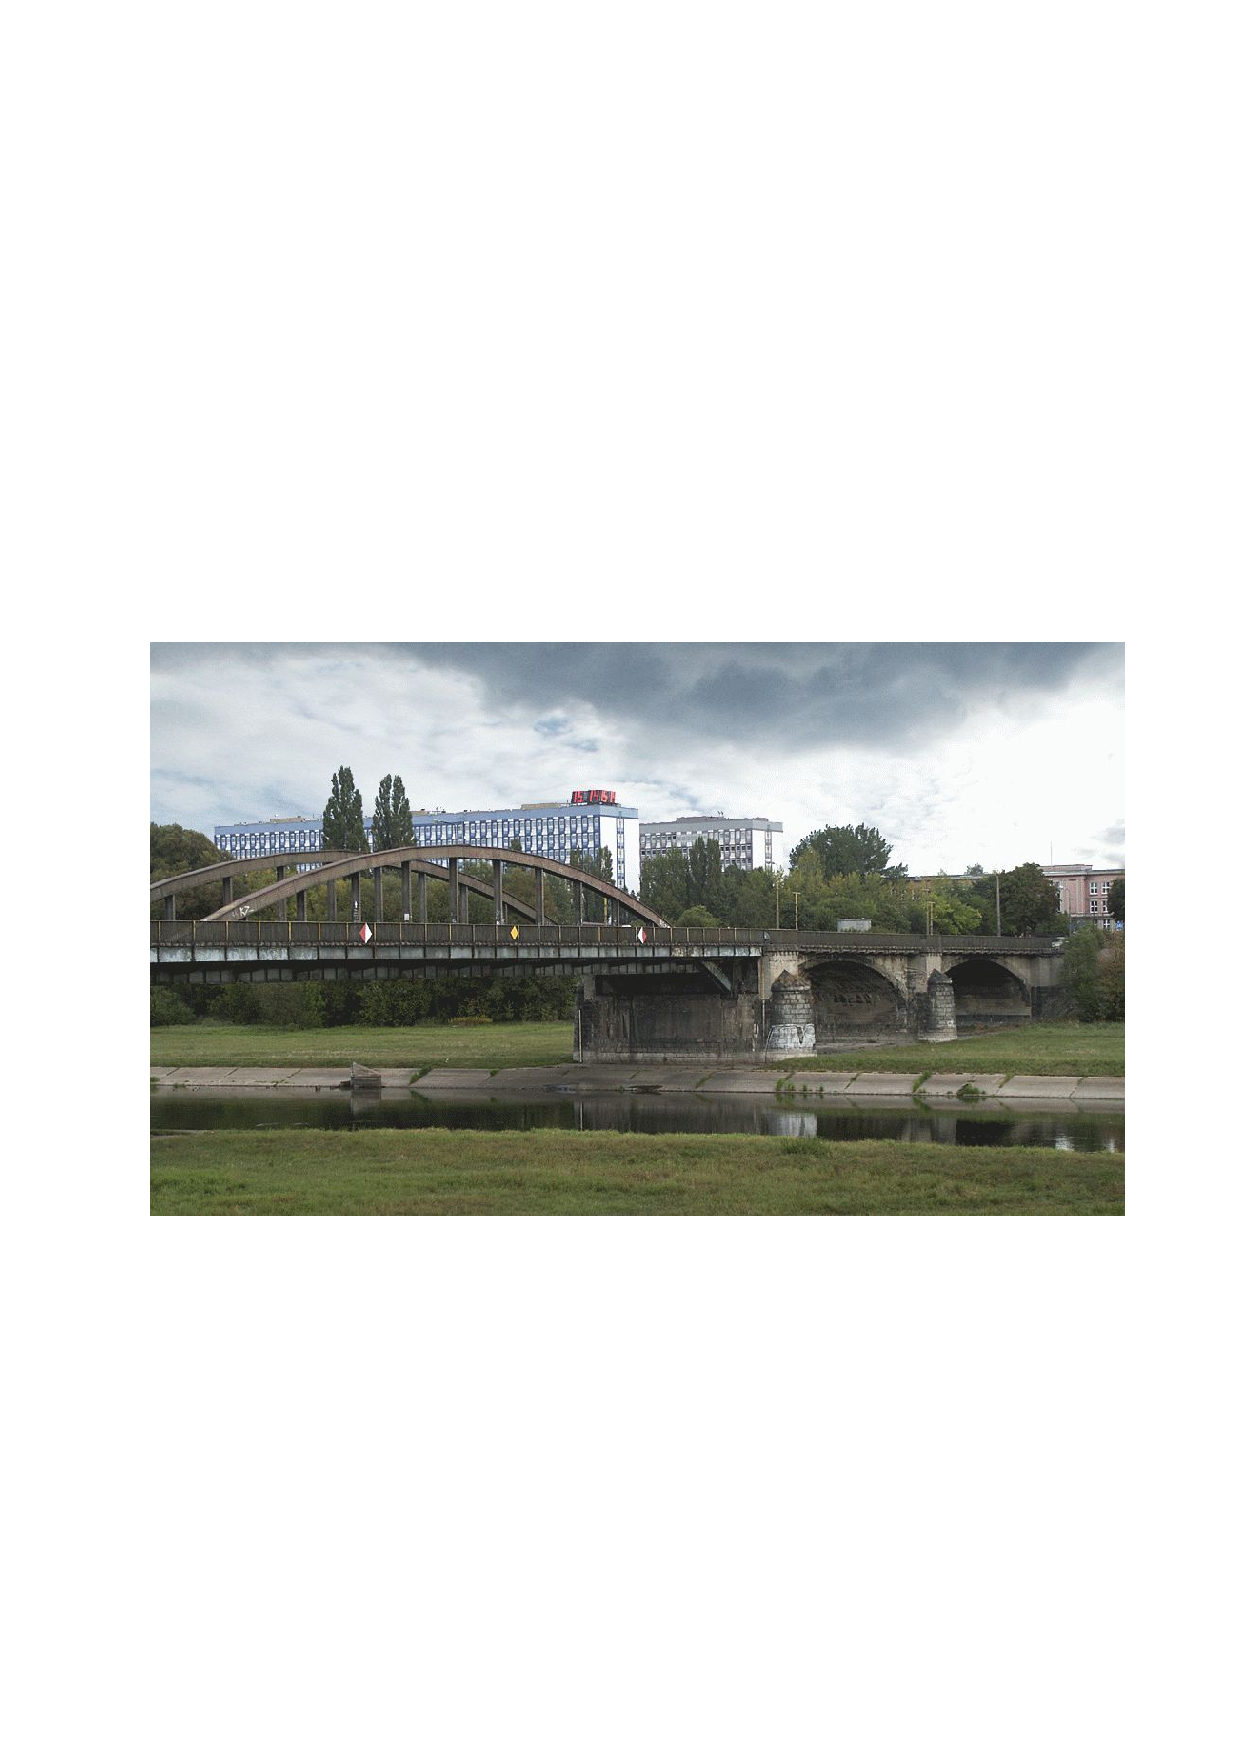
\includegraphics[width=8cm]{figures/cw-pp.jpg}
\end{center}
\caption{Budynki Instytutu Informatyki Politechniki Poznańskiej.}\label{rys:cwpp}
\end{figure}



\section{Wstawianie tablic}

Nowicjuszom polecam zrobienie tablic np.~w~Open Office i ich eksport do pliku
graficznego (lub PDF). Zaawansowani mogą spróbować wykonać je bezpośrednio
w \LaTeX{}u. Ważne jest, że nagłówki zwykle umieszcza się nad, a nie pod
obiektem (jak ma to miejsce w przypadku rysunków). Przykładowa tablica~\ref{tab:przyklad}
na stronie~\pageref{tab:przyklad} prezentuje jak to wygląda w kodzie.

\begin{table}
\caption{Przykład prostej tabeli.}\label{tab:przyklad}
\begin{center}
    \begin{tabular}{l | c}
    artykuł & cena [zł] \\
    \hline
    bułka   & $0.4$ \\
    masło   & $2.5$ \\
    \end{tabular}
\end{center}
\end{table}



\section{Bibliografia}

Polecam pakiet Bib\TeX, który ułatwia znakomicie zapis i spójne formatowanie
pozycji bibliograficznych. W kodzie źródłowym (plik \texttt{references.bib}) znajduje
się parę przykładów. Cytowanie z tekstu pracy uzyskujemy przy pomocy
polecenia \texttt{cite}. Przykładowo, Weiss i Stefanowski opisują system
Carrot$^2$ w pracy~\cite{stefanowski_weiss_awic2003}.



\subsection{Materiały instruktażowe}

Dokumentacji do systemu \LaTeX{} jest mnóstwo (zarówno w internecie, jak i~drukowanej).
Ten podręcznik wydaje się dobrym startem: \url{http://www.gust.org.pl/PDF/lshort2e.pdf}.


